\documentclass[12pt, a4paper]{article}
\usepackage[utf8]{inputenc}
\usepackage[portuguese]{babel}
\usepackage{color}
\usepackage{graphicx}
\usepackage{ulem}
\usepackage[utf8]{inputenc}
\title{A Vida do Suricata}
\author{João António-dos-Santos}
\date{\today}
\begin{document}

\maketitle
\section{Sobre o Suricata}
O \textbf{suricata}, também chamado de \textbf{suricato} ou \textbf{suricate} (\textit{Suricata suricatta}) é um pequeno mamífero da família \textit{Herpestidae}, nativo do deserto
do Kalahari. Estes animais têm cerca de meio metro de comprimento
(incluindo a cauda), em média 730 gramas de peso, e pelagem acastanhada. Têm garras afiadas nas patas, que lhes permitem escavar a superfície do ch\~ao e dentes afiados para penetrar nas carapaças quitinosas das suas presas. \textcolor{red} {Outra característica distinta é a sua capacidade de
se elevarem nas patas traseiras, utilizando a cauda como terceiro apoio.}
\section{Características gerais}
\subsection{Alimentação}
Alimenta-se principalmente de insetos (cerca de 82 \%): larvas de escaravelhos e de borboletas; também ingerem milípedes, aranhas, escorpi\~oes, pequenos vertebrados (répteis, anfíbios e aves), ovos e matéria vegetal. \uline {S\~ao relativamente imunes ao veneno} das najas e dos
escorpi\~oes, sendo estes, inclusive, um dos alimentos que mais apreciam.
\begin{figure}
\centering
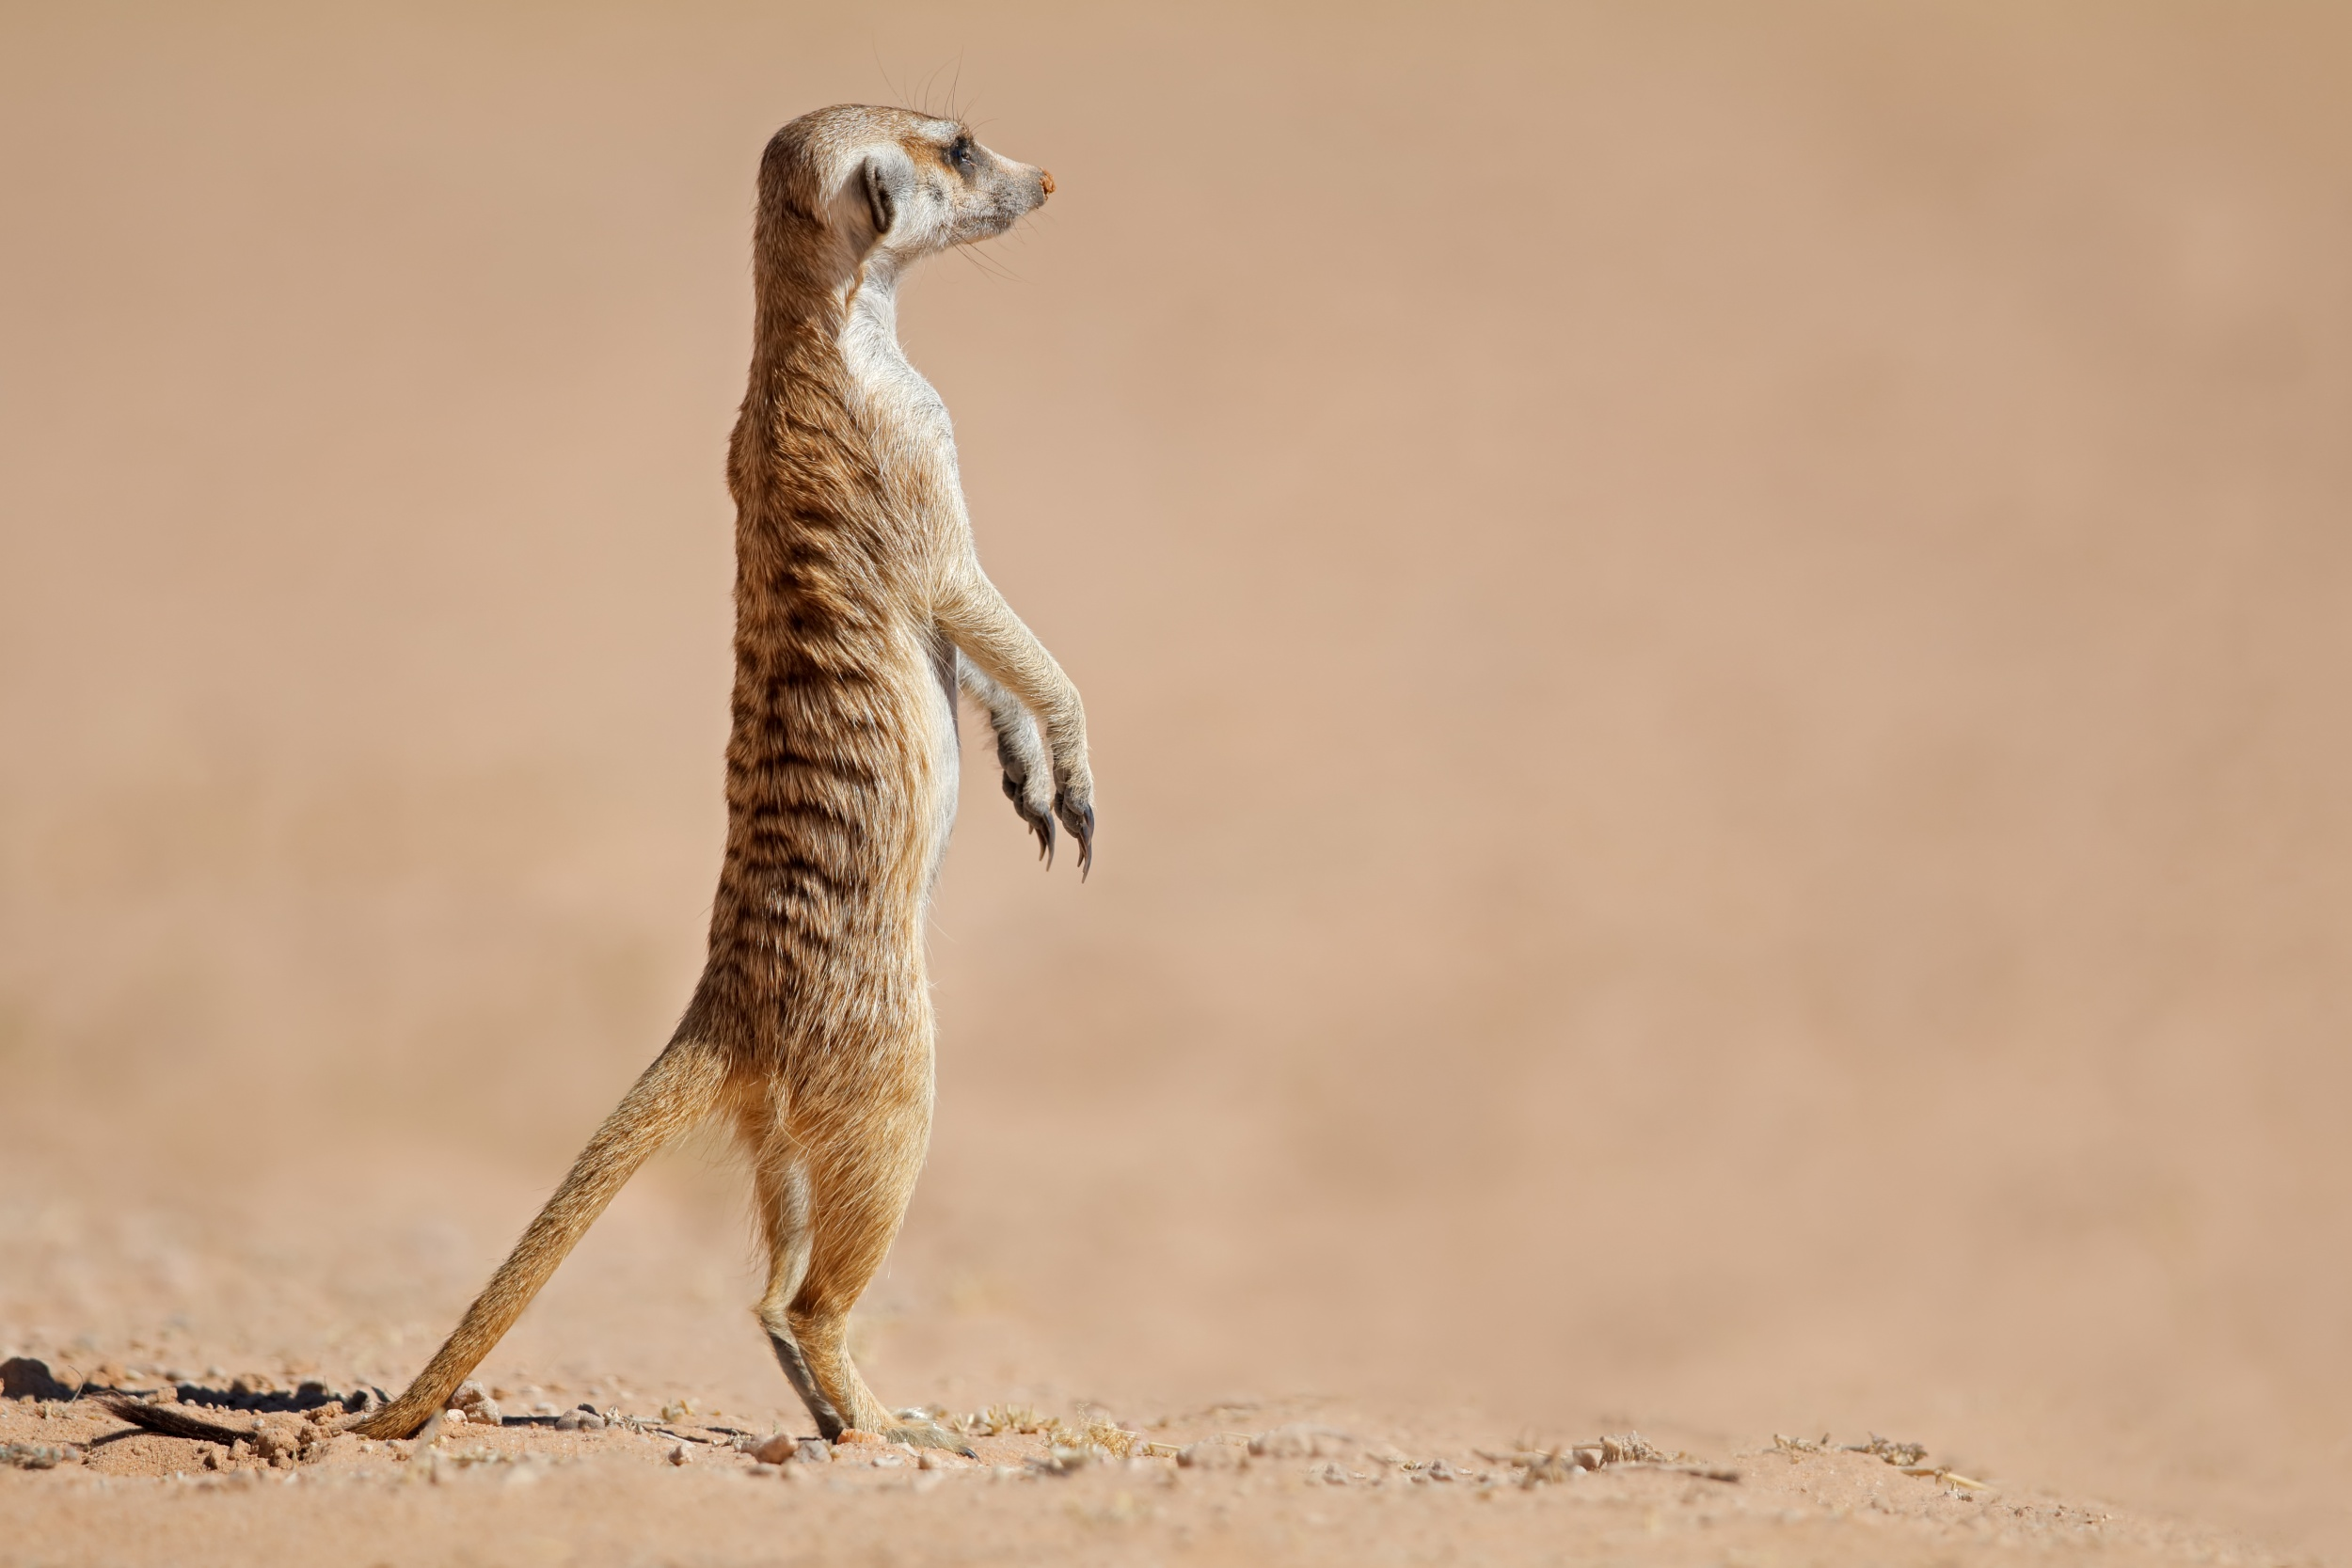
\includegraphics[scale=0.2]{suricata.jpg}
\caption{suricata}
\end{figure}

\end{document}